\subsection{Explain how AARB affects handling}
Active anti-roll bars (AARB) are a a new trend on modern vehicles that is being used more often recently. The goal behind it is to decrease the rolling of the vehicle to improve ride comfort, but more importantly to improve the handling of the vehicle.
To do so, the AARB acts as if one added extra springs between the axle and the body. So the forces on the tires will be amplified (i.e. the outer tire, which is being pushed to the ground will be pushed even more, while the inner tire will be pulled up more). This might cause wheel lift in extreme cases, and the AARB should account for that.

When it comes to the comfort, an AARB decreasing roll of the passenger compartment during maneuvers will indeed improve the ride comfort of the passenger. Moreover, while normal driving on an uneven road, the vehicle will be change its rolling stiffness to maintain a smooth ride while going over imperfections on the road like bumps or potholes.

As for the handling, the AARB changes the roll stiffness of each axle independently to achieve the desired roll of the vehicle. If one considers one of the axles, increasing the roll stiffness will cause a higher load transfer between the left and right side of the vehicle. Due to the degenerative relation between $F_Z$ and the cornering stiffness in the tires, for the same $\Delta F_z$, the cornering stiffness of the inner tire will decrease more than the increase of the cornering stiffness of the outer tire. This will decrease the overall cornering stiffness of the axle. If the axle was in front, this will make the car more understeered. If the axle is in the back, the vehicle will become less understeered. By choosing  
a distribution between the front and rear stiffnesses, one can control the understeer gradient of the vehicle and change its handling characteristics.

\subsection{Implement AARB and reduce roll gradient to 70\%}

The AARB increases the stiffness on one axle by applying a torque that compresses the suspension on one side, and elongates it on the other. To increase the roll stiffness of the vehicle, the AARB should "push down" the outer tyres and "pull up" the inner. This increases the roll stiffness of the vehicle and reduces the body roll during cornering. 

To find the magnitude of the torque that needs to be applied, a moment balance is done about the RC point of the front and rear axles during steady state cornering. Steady state was assumed for simplicity.  

\begin{align*}
    0 &= \textbf{M} + (I_{xx}+m_sh^2)\ddot{\phi} + k \Dot{\phi} + C \phi_{ref} - mg\phi -a_ym_sh_0\\
      \text{Steady } & \text{state cornering} \Rightarrow \ddot{\phi} =\dot{\phi} =0 \\
    0 &= \textbf{M} + C \phi_{ref} - mg\alpha -a_ym_sh_0\\
    \text{Where}&\\
    \phi_{ref} &= 0.7\cdot rollGradient\cdot a_y \text{ (to reduce roll gradient to 70\%)}
\end{align*}

% In the previous equations, it is assumed that $\ddot{\phi} = \Dot{\phi}=0$  because of steady state assumption. 

It is to note out that the generated moment, in bold, is the torque added by the AARB. This torque has to counteract the moments caused by the center of gravity and the fictitious lateral acceleration about the roll center. On the other hand, the passive stiffness of the passive anti-roll bar and the suspension is aiding the AARB.

The equation uses $\phi_{ref}$ since the aim is to use the AARB to get rid of the difference between the desired and actual roll, while the suspension would take care of the rest.

% i removed the passive roll bar bit cuz we dont know if there is.

To evaluate performance of the AARB, two simulations, with the AARB on and off, were ran with a ramp maneuver. To avoid transient behaviour, the ramp had a slope of $0.5[\degree/s]$ and the simulation time extended to 100s. Then, the roll angel $\phi$ was plotted against the lateral acceleration $a_y$. The slope of this plot is the roll gradient of the vehicle. As recommended by the teacher, this should be evaluated for lateral accelerations between $2-4[m/s^2]$. The results are shown below. 

\begin{figure}[H]
      \begin{minipage}[b]{0.49\linewidth}
      \centering
        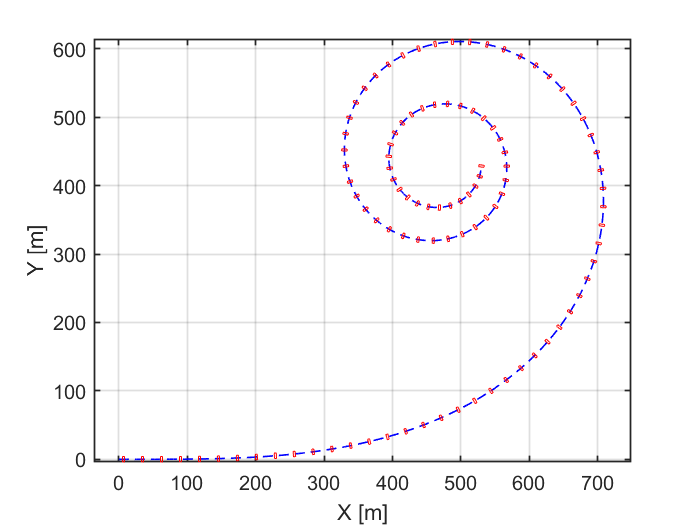
\includegraphics[width=\linewidth]{Figures/4_2_path.png}
        %  \caption*{Trajectory} 
        % \label{fig:2_4_l}
    \end{minipage} 
    \begin{minipage}[b]{0.49\linewidth}
    \centering
        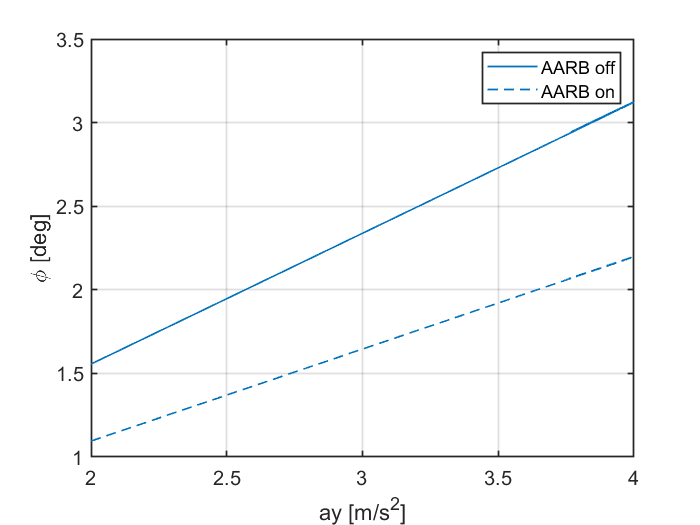
\includegraphics[width=\linewidth]{Figures/4_2_rollGrad.png}
        % \caption*{Yaw rate}
        % \label{fig:2_4_u}
    \end{minipage} 
    \caption{Path and Roll Gradient Comparison for a ramp steer input}
    %  \label{fig:headbodyrelmotion}
\end{figure}

\begin{figure}[H]
    \centering
    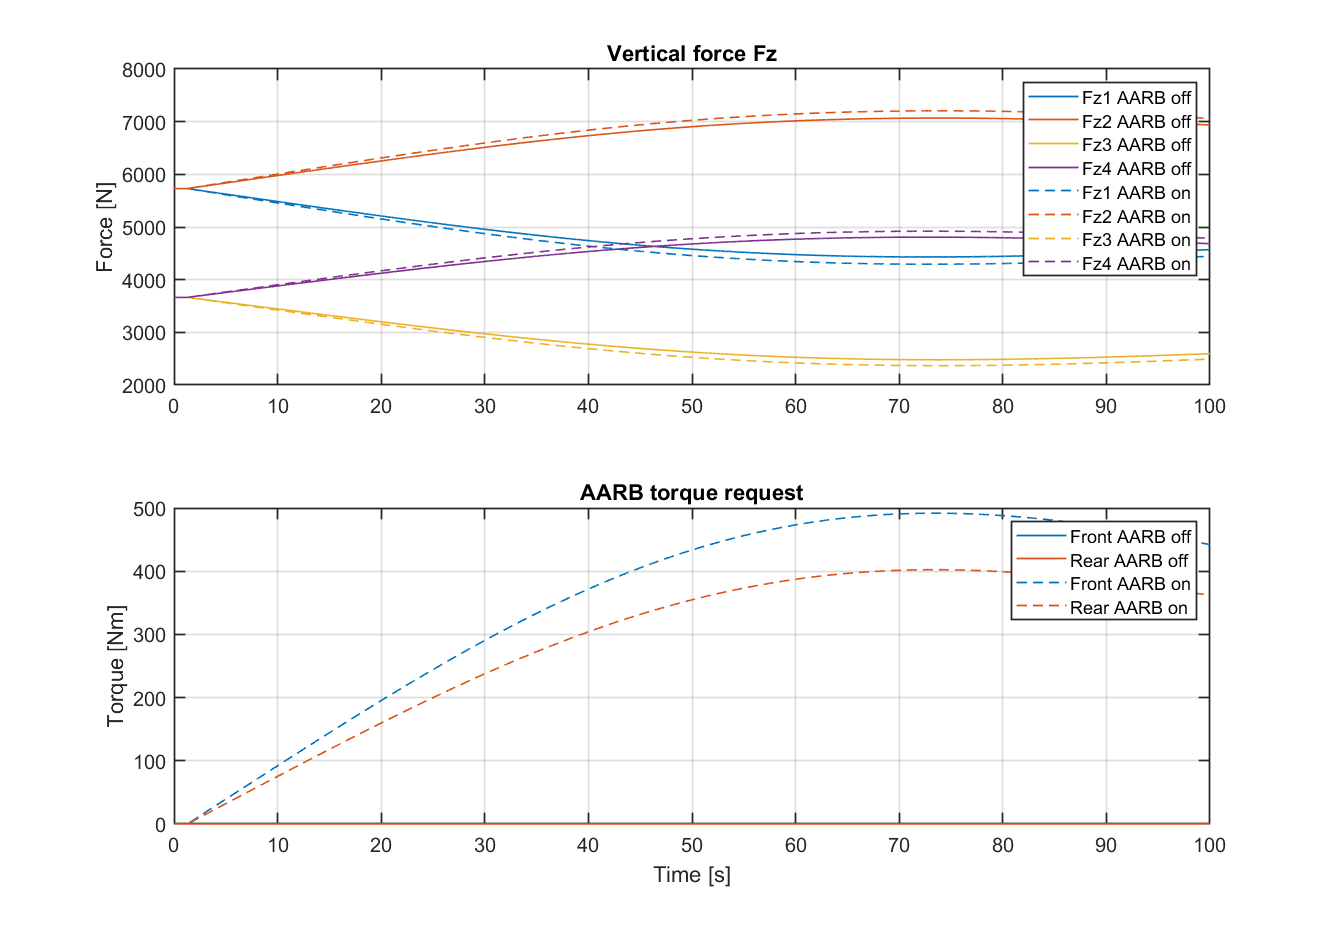
\includegraphics[width = \textwidth]{Figures/4_2_Fz.png}
    \caption{Tire Forces and required AARB torques}
    % \label{fig:my_label}
\end{figure}

\begin{table}[H]
    \centering
    \begin{tabular}{c|l}
         & Roll gradient $[\degree/(m/s^2)]$ \\\hline
        AARB off & 0.7850 \\
        AARB on &   0.5521 (70.33\%)
    \end{tabular}
    \caption{Roll gradient values}
    \label{tab:my_label}
\end{table}

As shown by the table above, the AARB seceded to bring the roll gradient of the vehicle to near $70\%$ of the original value. To test if this control method works for other percentages, it was tested for $50\%$ and $60\%$ as well and it produces similar results ($50\%$ and $60\%$ $\pm 0.4\%$). The small error might be due to $\ddot{\phi}$ and $\dot{\phi}$ not actually being 0. The non-linearity of the tyres might also have had an affect. 

\subsection{How can AARB affect transient behaviour}

As discussed before, changing the stiffness of the front and rear axles can make the vehicle more or less understeer. In the simulation, This was achived by changing the roll stiffness distribution $\lambda_c\phi$. To test this, three  simulations , AARB off, AARB induced understeer and AARB induced oversteer, were run with a step steer of $140\degree$ amplitude.  The resuts are shown below.

\begin{table}[H]
    \centering
    \begin{tabular}{c|c|c}
                    & understeer & oversteer\\\hline
         $\lambda_{c\phi}$ & 1.1  & -0.1\\
          $c_{\phi f}$ & $c_\phi\lambda_c$ & 0\\
          $c_{\phi r}$ & 0 &$c_\phi(1-\lambda_{c\phi})$
    \end{tabular}
    \caption{Controller input parameters for understeer and oversteer}
    \label{tab:my_label}
\end{table}

The parameters in the table above were, due to time constraints, found via trial and error until the required handling behaviour was achieved. 

\begin{figure}[H]
\begin{minipage}[b]{0.49\linewidth}
    \centering
    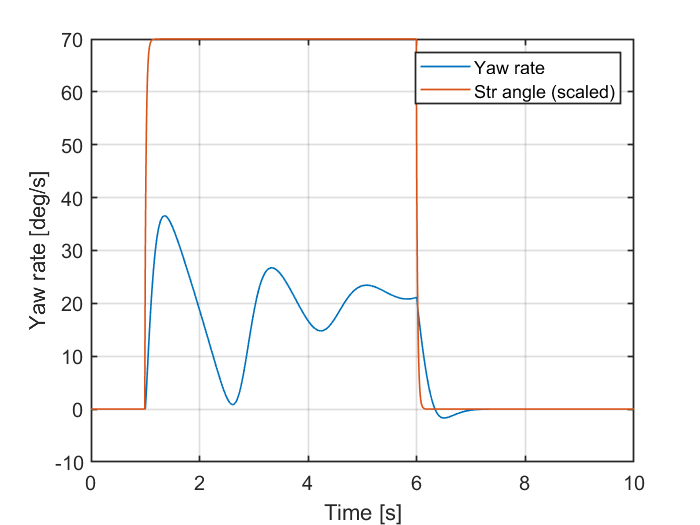
\includegraphics[width = \textwidth]{Figures/4_3_normal_140.png}
    \caption{AARB off}
\end{minipage}
\begin{minipage}[b]{0.49\linewidth}
    \centering
    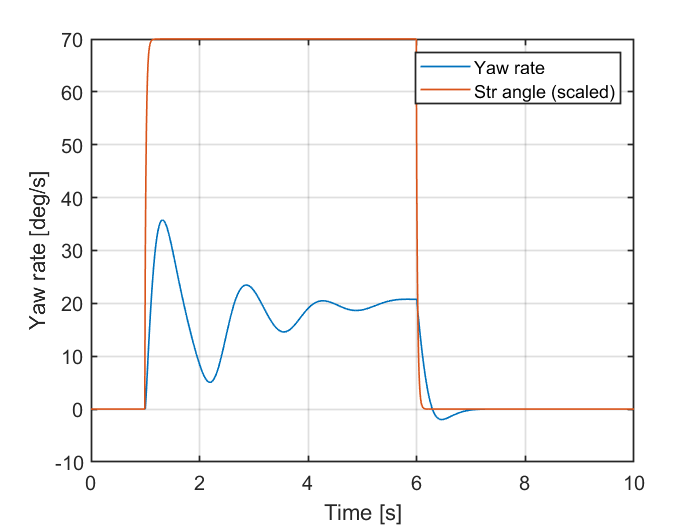
\includegraphics[width = \textwidth]{Figures/4_3_understeer_140.png}
    \caption{AARB induced understeer}
\end{minipage}
\begin{minipage}[b]{\linewidth}
    \centering
    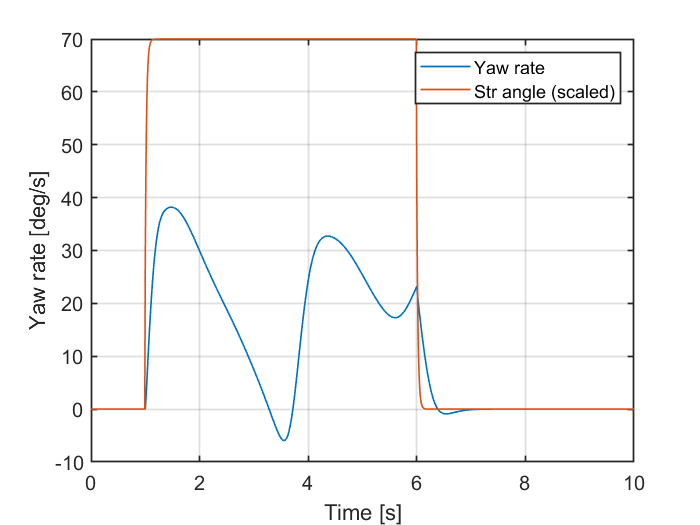
\includegraphics[width = 0.49 \textwidth]{Figures/4_3_oversteer_140.png}
    \caption{AARB induced oversteer}
\end{minipage}
\caption{Three simulations for step steer with 140$\degree$ amplitude}
\end{figure}

As can be seen in the figures above, the understeer case stabilises fastest. Moreover, the over steer case actually reaches a negative yaw rate for a positive steering angle and takes longer to stabilise. 

\subsection{Make vehicle understeer in SWD maneuver}

The same controller found in the task above was used here with for the SWD maneuver with the steering amplitude range SWD $\in[60,300]\degree$. The results were that the vehicle passed the test for the entire range. To see how the behaviour has changed, a simulation was run for steering amplitude $140\degree$ with the results shown below. 

\begin{figure}[H]
\begin{minipage}[b]{0.49\linewidth}
    \centering
    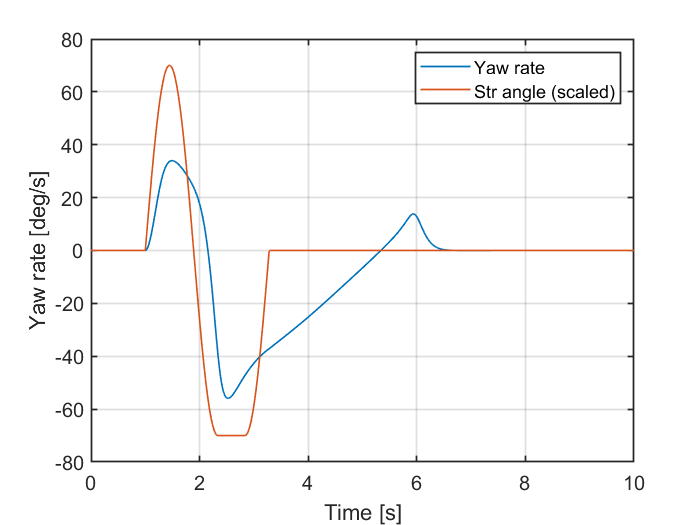
\includegraphics[width=\textwidth]{Figures/4_4_yaw_normalSteer_140deg.png}
    \caption{AARB off}
    \label{fig:my_label}
\end{minipage}
\begin{minipage}[b]{0.49\linewidth}
    \centering
    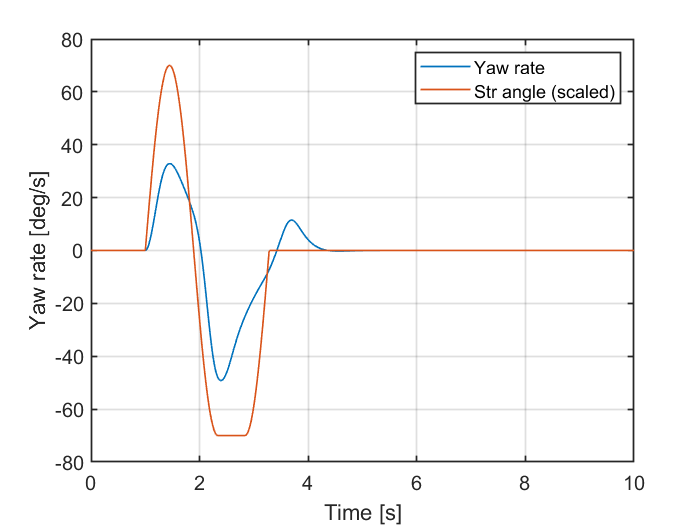
\includegraphics[width=\textwidth]{Figures/4_4_yaw_underSteer_140deg.png}
    \caption{AARB induced understeer}
    \label{fig:my_label}
\end{minipage}
\begin{minipage}[b]{0.9\linewidth}
    \centering
    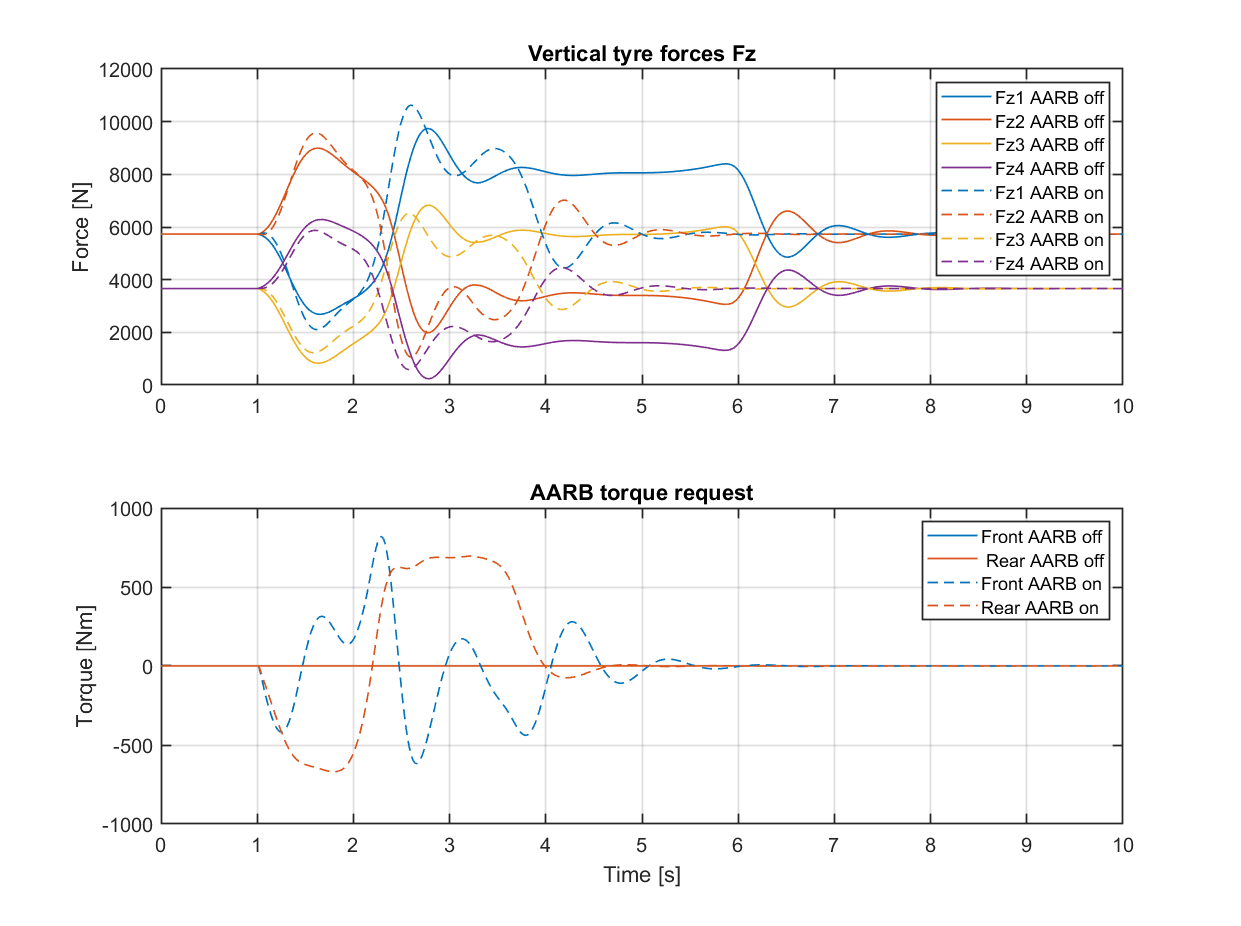
\includegraphics[width=\textwidth]{Figures/4_4_Fx_MxReq.png}
    \caption{Comparison between tyre forces for SWD with steering amplitude 140$\degree$}
\end{minipage}
\end{figure}

As seen above, the AARB makes the vehicle more stable through inducing understeer. This is apparent as the yaw rate returns to 0, and the vertical tyre forces stabilise, faster than with AARB off. 



